% \documentclass{article}
% \usepackage{graphicx} % Required for inserting images
% \usepackage{enumitem}
% \usepackage{parskip}

% \usepackage{caption}
% \usepackage{subcaption}


% \title{PHYS 506 - Experiment 2}
% \author{Luke Abanilla, Eben Quenneville, Augustus Vigorito}
% \date{November 2024}

\documentclass[prX,nofootinbib,notitlepage]{revtex4-1}
%------------------ Extending default LaTeX Structures -------------------
\usepackage{enumerate}
\usepackage{float}
\usepackage{caption}
\usepackage{hyperref}
\usepackage{subfiles}

%------------------------ Symbology \& Math ------------------------------
\usepackage{amsmath, amsthm, amssymb, amsfonts}
\usepackage{mathrsfs}
\usepackage{array}

%--------------------------- Graphics ------------------------------------
\usepackage[dvips]{graphics}
\usepackage{graphicx}
\usepackage{color}


%*************************************************************************
%****************************** Body *************************************
%*************************************************************************
\begin{document}

%************************ Document Settings ******************************

%---------------------- Bibliography Settings ----------------------------
\bibliographystyle{plain}

%--------------------------- Title ---------------------------------------
\title{PHYS 506 - Experiment 3 Semi-Report}

%----------------------- Author Information ------------------------------
\author{Luke Abanilla}
\author{Eben Quenneville}
\author{Augustus Vigorito}
\affiliation{Department of Physics, University of New Hampshire,
Durham, NH 03824, USA}
% \begin{document}
\date{December 2024}

\maketitle

\section{Theoretical Background}

\textbf{Use the work you did in the Problems 2 and 4, and any other information necessary to write about the Theoretical Background section should discuss the physics of the experiment, independent of the particulars of the measurement device(s) used to perform the experiment. (This mock-up theoretical background section should probably be approximately two or three paragraphs.)}

\textbf{Recall that a Theoretical Background Section should discuss the physics of the experiment. This will require derivations of the equations you will use to analyze your results, and you will need to derive these relevant equations in this section.}

\textbf{ \underline{Note:} The derivations you give should start from some well-known physics equations or principles and work to a final result. Rather than showing each and every step and algebraic manipulation involved in derivations, focus on giving more of an outline of the derivations (in words) and present/typeset only "milestone equations" (i.e., the important sub-results in the  derivation which lead you to the final result). Try not to skip too many steps, but basic algebraic rearrangements can be skipped. Do not go overboard with the derivation. Short, concise and to the point is much more effective.}

The charge and mass of an electron are incredibly important physical constants that appear throughout all of physics, from quantum mechanics to electromagnetism. Measuring the mass or charge of a single electron, however, is a very difficult task. Few of our instruments are capable of such a fine level of detail. A much easier task is to measure the ratio between the charge and mass. To do so, we need to find a method using information we already know. One way to do this is by using the Lorentz Force:
$$
\vec{F} = q\vec{v} \times \vec{B}
$$
where $\vec{F}$ is the force that a charge $q$ moving at a velocity $\vec{v}$ feels due to a magnetic field $\vec{B}$. The apparatus uses the Lorentz force to deflect the electron into uniform circular motion at a measurable radius $r$. There are still multiple values in this equation that need to be experimentally found. However, it is easier to measure force, velocity, and magnetic field than the very small charge of the electron. We determine these other values by using a combination of equations. To begin, we can derive the strength of the magnetic field due to the apparatus by applying the Biot-Savart law. Consider a circular loop of current of some known radius $R$ centered at the origin with $N$ coils. By the Biot-Savart Law, the magnetic field at a distance $x$ from the origin is given by
$$
\vec{B} = \frac{\mu_{0} I}{4 \pi ||\vec{r}||^{3} } \int\limits_{0}^{2\pi N}{d\vec{\ell} \times \vec{r}}
$$
where $\mu_0$ is the vacuum permeability constant, $I$ is the current flowing through the coil, and $\vec{r} = \vec{x} - \vec{R}$ is the vector from the point along the $x$-axis to some tiny arc of the coil $d\vec{\ell}$. Through careful algebraic manipulation and an application of the symmetry of the problem, it can be shown that 
$$
\vec{B} = \frac{\mu_{0} I N R^{2}}{2(x^{2} + R^{2})^{3/2}} \hat{x}
$$
If we add a second current loop in series with the other one, centered at $x = R$, then by the Principle of Superposition the magnetic field at a distance $x$ along the axis is given as
$$
B = \frac{\mu_{0} N I R^{2}}{2} \left( \frac{1}{(R^{2} + x^{2})^{3/2}} + \frac{1}{(R^{2} + (R-x)^{2})^{3/2}} \right)
$$
which, at a distance $x = R/2$, simplifies to 
$$
B = \left(\frac{4}{5}\right)^{3/2} \frac{\mu_{0} N I}{R}
$$
with uncertainty
$$
\delta B = \sqrt{\left(\frac{4}{5}\right)^{3} \left(\frac{\mu_{0} N }{R}\right)^{2} (\delta I)^{2} + \left(\frac{4}{5}\right)^{3} \left(\frac{- \mu_{0} N I}{R^{2}}\right)^{2} (\delta R)^{2}} 
$$
Now, to find the velocity, we use a conservation of energy approach. The apparatus applies an accelerating voltage of $V$ to the charge $q$, which, assuming that the electrons begin at rest, is converted into kinetic energy as
$$
qV = \frac{1}{2} m_{e}v^{2} \implies v = \sqrt{\frac{2qV}{m_{e}}}
$$
This velocity vector is perpendicular to the magnetic field by construction of the apparatus. For uniform circular motion, $F = mv^{2}/R$, so
$$
qvB = \frac{m_{e} v^2 }{r} \implies \frac{q}{m_e} = \frac{2V}{r^2 B^2}
$$
with uncertainty 
$$
\delta (e/m_e) = \frac{2}{r^2 B^2} \sqrt{\delta V^2 + \frac{4}{r^2 }\delta r^2 + \frac{4}{B^2 } \delta B^2}
$$
where $r$ is the radius of the circular motion. In order to experimentally determine the ratio of charge to mass, we need to gather data about voltage, magnetic field, and the radius of circular motion. The techniques used to find this data are described below.

\section{Experimental Methods}

\textbf{
Write about the experimental procedure and methods of this lab experiment, as if you were writing the Experimental Methods section of a formal lab report. (The mock-up experimental methods section should probably be two or more paragraphs).}

\textbf{Recall that the role of an Experimental Methods section is to give a description of the experiment you carried out. Write in your own words, but also try to maintain an air of formality in your writing. The experimental setup should not be a step-by-step recipe, but, rather, a set of text that describes all the various pieces of equipment used (ideally with diagrams, technical drawings, and/or circuit schematics), their arrangements, any calibrations, any settings, how the data was collected, and other information deemed necessary for the reader to understand what you did in this experiment.}

\newpage

% \begin{figure}
%     \begin{subfigure}
%         \centering
%         \includegraphics[width=0.5\linewidth]{}
%         \caption{Caption}
%         \label{fig:enter-label}        
%     \end{subfigure}

% \end{figure}

\begin{figure}[ht]
        \centering
        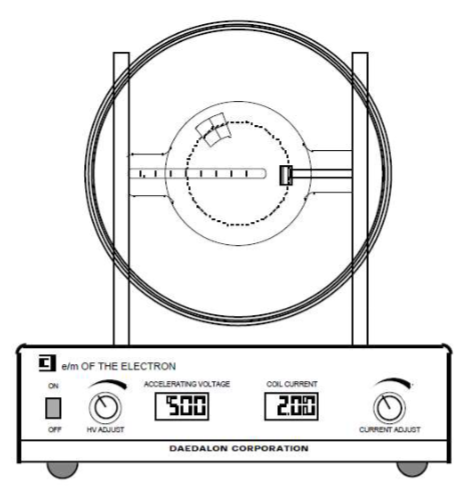
\includegraphics[width=0.5\linewidth]{exp 2 apparatus figure.png}
        \caption{\textit{e}/\textit{$m_l$} of the Electron Apparatus. Source: \cite{PHYS506}.}
        \label{fig:Figure 1}
\end{figure}

The apparatus (\ref{fig:Figure 1}) consists of three internal power supplies, each of which provide power to the anode, current to the coils, and accelerating voltage for the electron beam. Power to the anode, or filament, is fixed while the potential for the electron beam and the current to the coils are varied by the panel controls. These are measured by digital meters making it simpler to determine the forces acting on the electron beam. Within the bulb is an internal scale that measures in centimeters the diameter of the path of the electrons. Also included in the bulb is helium gas which fluoresces when hit by the moving electrons allowing for a much clearer view of the electron beam and better measurement. Additionally, at the end of the circular path of the electrons there is an electrode that absorbs the electrons after their path has been traced making measurements more accurate. 

\begin{figure}[h!]
    \centering
    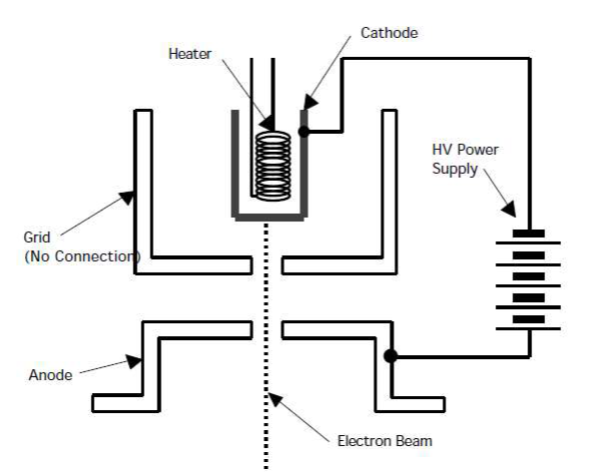
\includegraphics[width=0.5\linewidth]{exp 2 electron gun figure.png}
    \caption{Electron Gun Diagram. Source: \cite{PHYS506}.}
    \label{fig:Figure 2}
\end{figure}

Internally within the apparatus is an electron gun as shown above (\ref{fig:Figure 2}). At the top is a cathode which is connected to the negative terminal of the high voltage supply. This cathode is indirectly heated, emitting electrons some of which pass through a small aperture in the surrounding grid. An anode is connected to the bottom of the grid which accelerates the escaping electrons due to the potential difference between the cathode and the anode. Although most electrons hit the anode, some pass through forming the electron beam visible in the experiment. 

\section{Abstract}

\textbf{Write a mock-up Abstract for the work you did in this lab experiment, as if you were writing the Abstract to a formal lab report. (The mock-up abstract should probably be approximately a paragraph or two in length).}

\textbf{Recall that, generally speaking, an abstract is a kind of summary of your work designed to give the reader information regarding things like:}

\begin{itemize}
    \item Knowledge of the general (experimental) methods employed.
    \item Results of the main measurements, including values and errors.
    \item Relation to a theoretical prediction.
    \item Relation to other measurements.
\end{itemize}

\textbf{The idea of an abstract is to give your reader a short summary of the experiment performed, the methods used, and the results of your work, so that they can understand the experiment you performed (or problem you solved) without reading all the details of your work.}

\begin{abstract}
    The constants of electric charge (\textit{e}) and the mass of an electron (\textit{$m_l$}) are extremely small quantities to measure. However, the ratio of these constants can be calculated by curving an electron beam using a magnetic field and measuring the radius of curvature. This is achieved using a device known as an “\textit{e}/\textit{$m_l$} of the electron apparatus.” The apparatus consists of a vacuum in a bulb with an anode that ionizes helium such that the path of electrons emitting from the electron gun in the bulb is visible. The curvature in the beam of electrons is caused by a pair of coils known as “Helmholtz coils” which induce a magnetic field by running a known current through the coils. Using this method, the team accurately measured the ratio of \textit{e}/\textit{$m_l$}.
\end{abstract} 


%*************************** References **********************************
\begin{thebibliography}{99}

\section{References}

\bibitem{Lyons}
Lyons, L;
\textit{A Practical Guide to Data Analysis for Physical Science Students};
Cambridge Univ. Press; 1991.

% You should have several more references.
\bibitem{PHYS506}
Butbaia, Giorgi and Roberson, Matt;
\textit{PHYS506 - Experiment 2 Activity};
University of New Hampshire; 2024.

\end{thebibliography}

\end{document}